% Options for packages loaded elsewhere
\PassOptionsToPackage{unicode}{hyperref}
\PassOptionsToPackage{hyphens}{url}
%
\documentclass[
  Royal,
  times]{article}
\usepackage{amsmath,amssymb}
\usepackage{iftex}
\ifPDFTeX
  \usepackage[T1]{fontenc}
  \usepackage[utf8]{inputenc}
  \usepackage{textcomp} % provide euro and other symbols
\else % if luatex or xetex
  \usepackage{unicode-math} % this also loads fontspec
  \defaultfontfeatures{Scale=MatchLowercase}
  \defaultfontfeatures[\rmfamily]{Ligatures=TeX,Scale=1}
\fi
\usepackage{lmodern}
\ifPDFTeX\else
  % xetex/luatex font selection
\fi
% Use upquote if available, for straight quotes in verbatim environments
\IfFileExists{upquote.sty}{\usepackage{upquote}}{}
\IfFileExists{microtype.sty}{% use microtype if available
  \usepackage[]{microtype}
  \UseMicrotypeSet[protrusion]{basicmath} % disable protrusion for tt fonts
}{}
\makeatletter
\@ifundefined{KOMAClassName}{% if non-KOMA class
  \IfFileExists{parskip.sty}{%
    \usepackage{parskip}
  }{% else
    \setlength{\parindent}{0pt}
    \setlength{\parskip}{6pt plus 2pt minus 1pt}}
}{% if KOMA class
  \KOMAoptions{parskip=half}}
\makeatother
\usepackage{xcolor}
\usepackage[margin=1in]{geometry}
\usepackage{color}
\usepackage{fancyvrb}
\newcommand{\VerbBar}{|}
\newcommand{\VERB}{\Verb[commandchars=\\\{\}]}
\DefineVerbatimEnvironment{Highlighting}{Verbatim}{commandchars=\\\{\}}
% Add ',fontsize=\small' for more characters per line
\usepackage{framed}
\definecolor{shadecolor}{RGB}{248,248,248}
\newenvironment{Shaded}{\begin{snugshade}}{\end{snugshade}}
\newcommand{\AlertTok}[1]{\textcolor[rgb]{0.94,0.16,0.16}{#1}}
\newcommand{\AnnotationTok}[1]{\textcolor[rgb]{0.56,0.35,0.01}{\textbf{\textit{#1}}}}
\newcommand{\AttributeTok}[1]{\textcolor[rgb]{0.13,0.29,0.53}{#1}}
\newcommand{\BaseNTok}[1]{\textcolor[rgb]{0.00,0.00,0.81}{#1}}
\newcommand{\BuiltInTok}[1]{#1}
\newcommand{\CharTok}[1]{\textcolor[rgb]{0.31,0.60,0.02}{#1}}
\newcommand{\CommentTok}[1]{\textcolor[rgb]{0.56,0.35,0.01}{\textit{#1}}}
\newcommand{\CommentVarTok}[1]{\textcolor[rgb]{0.56,0.35,0.01}{\textbf{\textit{#1}}}}
\newcommand{\ConstantTok}[1]{\textcolor[rgb]{0.56,0.35,0.01}{#1}}
\newcommand{\ControlFlowTok}[1]{\textcolor[rgb]{0.13,0.29,0.53}{\textbf{#1}}}
\newcommand{\DataTypeTok}[1]{\textcolor[rgb]{0.13,0.29,0.53}{#1}}
\newcommand{\DecValTok}[1]{\textcolor[rgb]{0.00,0.00,0.81}{#1}}
\newcommand{\DocumentationTok}[1]{\textcolor[rgb]{0.56,0.35,0.01}{\textbf{\textit{#1}}}}
\newcommand{\ErrorTok}[1]{\textcolor[rgb]{0.64,0.00,0.00}{\textbf{#1}}}
\newcommand{\ExtensionTok}[1]{#1}
\newcommand{\FloatTok}[1]{\textcolor[rgb]{0.00,0.00,0.81}{#1}}
\newcommand{\FunctionTok}[1]{\textcolor[rgb]{0.13,0.29,0.53}{\textbf{#1}}}
\newcommand{\ImportTok}[1]{#1}
\newcommand{\InformationTok}[1]{\textcolor[rgb]{0.56,0.35,0.01}{\textbf{\textit{#1}}}}
\newcommand{\KeywordTok}[1]{\textcolor[rgb]{0.13,0.29,0.53}{\textbf{#1}}}
\newcommand{\NormalTok}[1]{#1}
\newcommand{\OperatorTok}[1]{\textcolor[rgb]{0.81,0.36,0.00}{\textbf{#1}}}
\newcommand{\OtherTok}[1]{\textcolor[rgb]{0.56,0.35,0.01}{#1}}
\newcommand{\PreprocessorTok}[1]{\textcolor[rgb]{0.56,0.35,0.01}{\textit{#1}}}
\newcommand{\RegionMarkerTok}[1]{#1}
\newcommand{\SpecialCharTok}[1]{\textcolor[rgb]{0.81,0.36,0.00}{\textbf{#1}}}
\newcommand{\SpecialStringTok}[1]{\textcolor[rgb]{0.31,0.60,0.02}{#1}}
\newcommand{\StringTok}[1]{\textcolor[rgb]{0.31,0.60,0.02}{#1}}
\newcommand{\VariableTok}[1]{\textcolor[rgb]{0.00,0.00,0.00}{#1}}
\newcommand{\VerbatimStringTok}[1]{\textcolor[rgb]{0.31,0.60,0.02}{#1}}
\newcommand{\WarningTok}[1]{\textcolor[rgb]{0.56,0.35,0.01}{\textbf{\textit{#1}}}}
\usepackage{longtable,booktabs,array}
\usepackage{calc} % for calculating minipage widths
% Correct order of tables after \paragraph or \subparagraph
\usepackage{etoolbox}
\makeatletter
\patchcmd\longtable{\par}{\if@noskipsec\mbox{}\fi\par}{}{}
\makeatother
% Allow footnotes in longtable head/foot
\IfFileExists{footnotehyper.sty}{\usepackage{footnotehyper}}{\usepackage{footnote}}
\makesavenoteenv{longtable}
\usepackage{graphicx}
\makeatletter
\def\maxwidth{\ifdim\Gin@nat@width>\linewidth\linewidth\else\Gin@nat@width\fi}
\def\maxheight{\ifdim\Gin@nat@height>\textheight\textheight\else\Gin@nat@height\fi}
\makeatother
% Scale images if necessary, so that they will not overflow the page
% margins by default, and it is still possible to overwrite the defaults
% using explicit options in \includegraphics[width, height, ...]{}
\setkeys{Gin}{width=\maxwidth,height=\maxheight,keepaspectratio}
% Set default figure placement to htbp
\makeatletter
\def\fps@figure{htbp}
\makeatother
\setlength{\emergencystretch}{3em} % prevent overfull lines
\providecommand{\tightlist}{%
  \setlength{\itemsep}{0pt}\setlength{\parskip}{0pt}}
\setcounter{secnumdepth}{-\maxdimen} % remove section numbering
% definitions for citeproc citations
\NewDocumentCommand\citeproctext{}{}
\NewDocumentCommand\citeproc{mm}{%
  \begingroup\def\citeproctext{#2}\cite{#1}\endgroup}
\makeatletter
 % allow citations to break across lines
 \let\@cite@ofmt\@firstofone
 % avoid brackets around text for \cite:
 \def\@biblabel#1{}
 \def\@cite#1#2{{#1\if@tempswa , #2\fi}}
\makeatother
\newlength{\cslhangindent}
\setlength{\cslhangindent}{1.5em}
\newlength{\csllabelwidth}
\setlength{\csllabelwidth}{3em}
\newenvironment{CSLReferences}[2] % #1 hanging-indent, #2 entry-spacing
 {\begin{list}{}{%
  \setlength{\itemindent}{0pt}
  \setlength{\leftmargin}{0pt}
  \setlength{\parsep}{0pt}
  % turn on hanging indent if param 1 is 1
  \ifodd #1
   \setlength{\leftmargin}{\cslhangindent}
   \setlength{\itemindent}{-1\cslhangindent}
  \fi
  % set entry spacing
  \setlength{\itemsep}{#2\baselineskip}}}
 {\end{list}}
\usepackage{calc}
\newcommand{\CSLBlock}[1]{\hfill\break\parbox[t]{\linewidth}{\strut\ignorespaces#1\strut}}
\newcommand{\CSLLeftMargin}[1]{\parbox[t]{\csllabelwidth}{\strut#1\strut}}
\newcommand{\CSLRightInline}[1]{\parbox[t]{\linewidth - \csllabelwidth}{\strut#1\strut}}
\newcommand{\CSLIndent}[1]{\hspace{\cslhangindent}#1}
\ifLuaTeX
  \usepackage{selnolig}  % disable illegal ligatures
\fi
\usepackage{bookmark}
\IfFileExists{xurl.sty}{\usepackage{xurl}}{} % add URL line breaks if available
\urlstyle{same}
\hypersetup{
  pdftitle={ActiveCA: Time Use Data from the General Social Survey of Canada to Study Active Travel},
  pdfkeywords={Active; mobility; walking; cycling; travel time;
time-use; General Social Survey},
  hidelinks,
  pdfcreator={LaTeX via pandoc}}

\title{ActiveCA: Time Use Data from the General Social Survey of Canada
to Study Active Travel}
\author{true \and true \and true}
\date{}

\begin{document}
\maketitle
\begin{abstract}
This paper describes \{ActiveCA\}, an open data product with Canadian
time use data. \{ActiveCA\} is an \texttt{R} data package that contains
analysis-ready data related to active travel spanning almost 40 years,
extracted from cycles 2 (1986), 7 (1992), 12 (1998), 19 (2005), 24
(2010), and 29 (2015) of Canada's General Social Survey. Active travel
is characterized by mode, with walking being part of every cycle and
bicycling starting in 1992. The attributes of active trips are the types
of locations of origins and destinations, the duration of trips, and
episode weights for expanding the trips to population-wide estimates.
Based on the year of the survey, a variety of locations are coded. In
earlier cycles, these include home, work or school, and other's home,
whereas in later cycles these are augmented with locations such as
grocery stores, restaurants, outdoor destinations, and others. The
geographical resolution includes the province and whether the episode
was in an urban or rural setting.
\end{abstract}

\section{Introduction}\label{introduction}

The objective of this paper is to introduce \{ActiveCA\}, an open data
product with time use data from Canada's General Social Surveys. Open
data products (ODPs) are the outcome of a process that transforms raw
data (open or not) into analysis-ready data, following a transparent
process in which all stages of development follow open principles
(Arribas-Bel et al. 2021). ODPs, while still open, differ from general
open data in their degree of ease of access, their heightened usability,
and potentially the value they add to the raw data.

\{ActiveCA\} provides analysis-ready data concerning active travel in
Canada spanning a period of almost 40 years. The source of these data is
Canada's program of General Social Surveys (GSSs). This program is
designed to provide cross-sectional data on topics of interest to
improve the well-being of Canadians. As part of this program, every five
to seven years the survey is done on the topic of time use. Concretely,
\{ActiveCA\} covers Cycles 2 (1986), 7 (1992), 12 (1998), 19 (2005), 24
(2010), and 29 (2015) of the GSS. Time use data in these surveys is
coded using a very fine grain, from time spent in chores, leisure, and
sleeping, to time spent working or at school. These surveys have proved
valuable in investigations of mobility and quality of life (Spinney,
Scott, and Newbold 2009), the relationship between active travel and
transit use (Lachapelle and Pinto 2016), and travel behavior and time
poverty (Kim et al. 2024), to name but a few examples.

For \{ActiveCA\} and using GSS Public Use Microdata Files (PUMFs), we
extracted all data needed to characterize active travel in Canada,
namely, episodes where the activity was identified as moving between an
origin and a destination, either by walking or cycling. Although
Statistics Canada offers Public Use Microdata Files and documentation
for the GSS program (see Canada 2024), accessing these files, and
preparing them for analysis is not a straightforward matter, given their
size and complexity. The process of extracting information of interest
from the source files is time-consuming, tedious, and challenging and/or
prone to error due to the expertise required to work with these files.
To create \{ActiveCA\} we collected, cleaned, and processed the cycles
of the GSS surveys concerning time use to make them ready for analysis.

\{ActiveCA\} is distributed as an \texttt{R} package with a number of
data objects and their documentation. \texttt{R} packages contain code,
data, and documentation in a standardized format that can be installed
by \texttt{R} users via a software repository, such as CRAN
(Comprehensive R Archive Network) or GitHub, which makes them an adroit
medium to distribute analysis-ready data.

Given the level of interest in active travel (e.g., McCurdy et al.
2023), reducing the barriers to using data contained in rich, but
difficult to access and use surveys, such as Canada's GSSs, is a worthy
endeavour that can only improve data-driven decisions in transportation,
urban, and health policy.

The rest of this paper discusses the sources of data, and the process
implemented to retrieve and package them. Then, we explain how to use
the package and show some selected examples of analysis to whet the
imagination of potential users. This ODP provides not only data that are
easy to use, but also all the code and documentation that make this a
reproducible research project. In summary, \{ActiveCA\} aims to
implement and inspire the best principles of open spatial sciences (Páez
2021; Brunsdon and Comber 2021).

\section{General Social Survey (GSS)
collection}\label{general-social-survey-gss-collection}

Statistics Canada (2024) conducts GSS surveys to obtain data on social
trends to track changes in Canadians' living conditions and well-being
over time. The series of survey on time use are used to understand how
Canadian residents spend and manage their time, and what factors
contribute to their happiness and stress. The GSS program was created in
1985, and is serialized to provide a collection of annual,
representative cross-sectional surveys.

The topics of the survey cycle every few years to cover topics that
include family, health, social identity, and every five to seven years
time use. The first Canadian time use survey done as part of the GSS
program was conducted in 1986, and the most recent was completed in
2015. These Time Use Surveys (Canada 2022) collect data on respondents'
participation and time spent on a wide range of everyday activities
using a 24-hour retrospective diary, with information on the location of
these activities (e.g.~at home, at work, etc.) and, for non-personal
activities, the people who were present with the respondent at the time
of the activity. In addition, time-use surveys also cover topics related
to leisure time, work-life balance, health, commuting, culture and
sports, and many others.

The Public Use Microdata are released by Statistics Canada in two files:
a \emph{Main File} and an \emph{Episode File}. The files are linked by
keys that identify households, individuals, and episodes (i.e.,
activities) conducted by individuals. We discuss these files in more
detail in the following section.

\subsection{The Main File}\label{the-main-file}

The Main File of the time use survey compiles a large array of
aggregated data, summarizing the answers to the questionnaire that
describe households and individuals, as well as derived variables that
summarize the respondents' use of time use across different activities,
locations, and social interactions. This file documents the time and
duration that respondents allocate to each activity and location. The
Main File provides a overview of daily routines and social dynamics, not
focusing on individual activity episodes. Additionally, this file
categorizes activities into bigger groups and subcategories,
facilitating the data's analytical utility with additional metrics such
as total transit time, time spent with household members, and counts of
activities and episodes.

Table \ref{tab:main-2015-unprocessed} shows the first ten rows and first
six variables of the GSS PUMF 2015 Main File (Cycle 29). Each row in the
table correspond to a survey respondent, while the columns refer the
following information: record identification (\texttt{PUMFID}), the
person's weight (\texttt{WGHT\_PER}), the month the survey data was
collected (\texttt{SURVMNTH}), the respondent's age group
(\texttt{AGEGR10}), the respondent's sex (\texttt{SEX}), and the
respondent's marital status (\texttt{MARSTAT}).

The Main File of the 2015 GSS surveys includes a total of 17,390
respondents, representing 29,766,399 individuals and 848 variables. For
discrete variables, Statistics Canada has assigned specific codes to the
possible values, with each code accompanied by a label. For instance, in
the case of the variable \texttt{SURVMNTH}, a value of \texttt{1} means
\texttt{January\ 2016}, 2 means \texttt{February\ 2016}, 3 corresponds
to \texttt{March\ 2016}, and so on.

As shown in Table \ref{tab:main-2015-unprocessed}, the variables are not
labeled. Adittionaly, the format of the tables (comma-separated values)
does not allow for the specification of variable types (whether a
variable is continuous or discrete), which can lead to mistakes analysts
who have limited experience working with PUMFs.

\begingroup\fontsize{8}{10}\selectfont

\begin{ThreePartTable}
\begin{TableNotes}
\item \textit{Note: } 
\item Legend: `PUMFID`: record identification. `WGHT\_PER`:  person weight. `SURVMNTH`: survey month of data collection. `AGEGR10`: age group of the respondent. `SEX`: sex of the respondent. `MARSTAT`: marital status of the respondent.
\end{TableNotes}
\begin{longtable}[t]{cccccc}
\caption{\label{tab:gss-main-file-2015}\label{tab:main-2015-unprocessed}Visualization of the first ten lines and first six columns of the Main File of the 2015 GSS.}\\
\toprule
PUMFID & WGHT\_PER & SURVMNTH & AGEGR10 & SEX & MARSTAT\\
\midrule
10000 & 616.6740 & 7 & 5 & 1 & 5\\
10001 & 8516.6140 & 7 & 5 & 1 & 1\\
10002 & 371.7520 & 1 & 4 & 2 & 1\\
10003 & 1019.3135 & 3 & 6 & 2 & 5\\
10004 & 1916.0708 & 9 & 2 & 1 & 6\\
\addlinespace
10005 & 1952.2015 & 4 & 1 & 1 & 6\\
10006 & 5761.5528 & 8 & 1 & 1 & 6\\
10007 & 466.0426 & 6 & 5 & 2 & 3\\
10008 & 2479.2991 & 2 & 2 & 2 & 1\\
10009 & 1436.1641 & 8 & 6 & 1 & 3\\
\bottomrule
\insertTableNotes
\end{longtable}
\end{ThreePartTable}
\endgroup{}

\subsection{The Episode File}\label{the-episode-file}

The episode is a much bigger file that records detailed data for each
activity episode reported by respondents. Each episode represents a
single activity and its duration, and the sum of all episodes throughout
the day adds up to 24 hours. Each entry in this file includes the start
and end times of the activity, the duration, location, and accompanying
social context, informing when and where activities occurred and with
whom. The focus of the Episode File is not on the characteristics of the
respondents, but on the characteristics of the activities, and the data
are structured around the numerous activity instances that compose a day
of the respondent. Although respondent-specific characteristics are not
included within the Episode File, it is possible to link the Main File
and the Episode File by using a key present in both the Main and Episode
Files.

Similar to Table \ref{tab:main-2015-unprocessed}, which displayed an
example of the Main File structure, Table \ref{tab:ep-2015-unprocessed}
presents the first seven episodes for the record identification number
\texttt{10041} and some variables from the GSS PUMF 2015 Episode File
(Cycle 29). Each row in the table corresponds to an episode associated
with the specified record identification (\texttt{PUMFID\ =\ 10041}),
including the episode's weight (\texttt{WGHT\_EPI}), episode number
(\texttt{EPINO}), activity code (\texttt{TUI\_01}), episode duration
(\texttt{DURATION}), and episode location (\texttt{LOCATION}).

In total, the Episode File of the 2015 GSS surveys contains 274,108
records, representing 461,837,622 episodes and 527 variables detailing
the episodes. Similar to the Main File, Statistics Canada has created
codes for the discrete variables, with each value corresponding to a
label.

In the case illustrated in Table \ref{tab:ep-2015-unprocessed}, this
respondent began the diary description by sleeping at home
(\texttt{TUI\_01\ =\ 1} and \texttt{LOCATION\ =\ 300}) for 210 minutes,
followed by 40 minutes of personal hygiene (\texttt{TUI\_01\ =\ 2}). The
respondent then spent 15 minutes on personal care activities, such as
getting ready for school, supervising homework, reading, playing,
reprimanding, or providing educational or emotional support, as
indicated by \texttt{TUI\_01\ =\ 27}. Next, they recorded a travel
episode, walking for 15 minutes (\texttt{TUI\_01\ =\ 7} and
\texttt{LOCATION\ =\ 315}), where both the origin and destination were
their home. Such trips, where the journey starts and finishes at home,
can be classified as recreational or leisure trips. Next, the respondent
spent 3 hours searching for a job (\texttt{TUI\_01\ =\ 9}), took a
15-minute lunch break (\texttt{TUI\_01\ =\ 6}), and then cleaned the
house (\texttt{TUI\_01\ =\ 18}) for two hours. Table
\ref{tab:ep-2015-unprocessed} displays only six variables out of the 527
available. As shown, since the dataset does not label the variable
values, decoding them can be both time-consuming and challenging.

\begingroup\fontsize{8}{10}\selectfont

\begin{ThreePartTable}
\begin{TableNotes}
\item \textit{Note: } 
\item Legend: `PUMFID`: record identification. `EPINO`: episode number. WGHT\_EPI: episode's weight. TUI\_01: activity code. DURATION: episode's duration. LOCATION: episode's location.
\end{TableNotes}
\begin{longtable}[t]{cccccc}
\caption{\label{tab:gss-epi-file-2015}\label{tab:ep-2015-unprocessed}Visualization of the seven first episodes of the record number `10041`.}\\
\toprule
PUMFID & EPINO & WGHT\_EPI & TUI\_01 & DURATION & LOCATION\\
\midrule
10041 & 1 & 1353.818 & 1 & 210 & 300\\
10041 & 2 & 1353.818 & 2 & 40 & 300\\
10041 & 3 & 1353.818 & 27 & 15 & 300\\
10041 & 4 & 1353.818 & 7 & 15 & 315\\
10041 & 5 & 1353.818 & 9 & 180 & 300\\
\addlinespace
10041 & 6 & 1353.818 & 6 & 15 & 300\\
10041 & 7 & 1353.818 & 18 & 120 & 300\\
\bottomrule
\insertTableNotes
\end{longtable}
\end{ThreePartTable}
\endgroup{}

\section{Data extraction}\label{data-extraction}

For each selected cycle of the GSS surveys, we reviewed the Episode
Files to identify episodes of movement that involved walking or cycling.
This allowed us to select the activities immediately before and after
the movement episode. After that, we labeled the code variables with
their appropriate descriptions, identifying each origin and destination,
mode of travel, time spent in the active trip, as well the province and
urban classification of the episode.

The active trips (walking and cycling) were identified by their
corresponding activity codes, accounting for differences between the
survey cycles. Identifying the preceding and succeeding activities of
each activity episode helps to understand the motivation for the trip
and also determine the origin and destination of the trips.

For each GSS Main File, we selected socioeconomic variables to help
profile the individuals engaged in active trip episodes. We included key
socioeconomic variables such as the respondent's age group, sex, marital
status, and number of children, among others. After this, as we did with
the Episode Files, we labeled the code variables with their appropriate
descriptions.

\section{How to use \{ActiveCA\}}\label{how-to-use-activeca}

This section presents some potential applications of the \{ActiveCA\} R
package. In fact, we expect that the application of this package to
extend beyond our pre-imagined range of uses.

To start the demonstration, it is first necessary to install the
package. The code chunk below demonstrates how to install the
\{ActiveCA\} package in R:

\begin{Shaded}
\begin{Highlighting}[]
\ControlFlowTok{if}\NormalTok{(}\SpecialCharTok{!}\FunctionTok{require}\NormalTok{(}\StringTok{"ActiveCA"}\NormalTok{, }\AttributeTok{character.only =} \ConstantTok{TRUE}\NormalTok{)) \{}
\NormalTok{      remotes}\SpecialCharTok{::}\FunctionTok{install\_github}\NormalTok{(}\StringTok{"dias{-}bruno/ActiveCA"}\NormalTok{)}
\NormalTok{\}}
\end{Highlighting}
\end{Shaded}

After installing the \{ActiveCA\} R package, you can load it using the
following code:

\begin{Shaded}
\begin{Highlighting}[]
\FunctionTok{library}\NormalTok{(ActiveCA)}
\end{Highlighting}
\end{Shaded}

The documentation of the package can be accessed by running
\texttt{?ActiveCA} in \texttt{R}. The documentation includes a
description of the package, information about the authors, contributors,
and maintainers, and an overview of all pre-processed data sets included
in the package.

Figure \ref{fig:walking_documentation} displays the documentation for
the walking episodes from the 2015 GSS (\texttt{walking\_2015.rda}). The
documentation provides a brief description of the dataset, instructions
on how to load the package, as well as details about the file format and
descriptions of all variables (already labeled).

\begin{figure}

{\centering 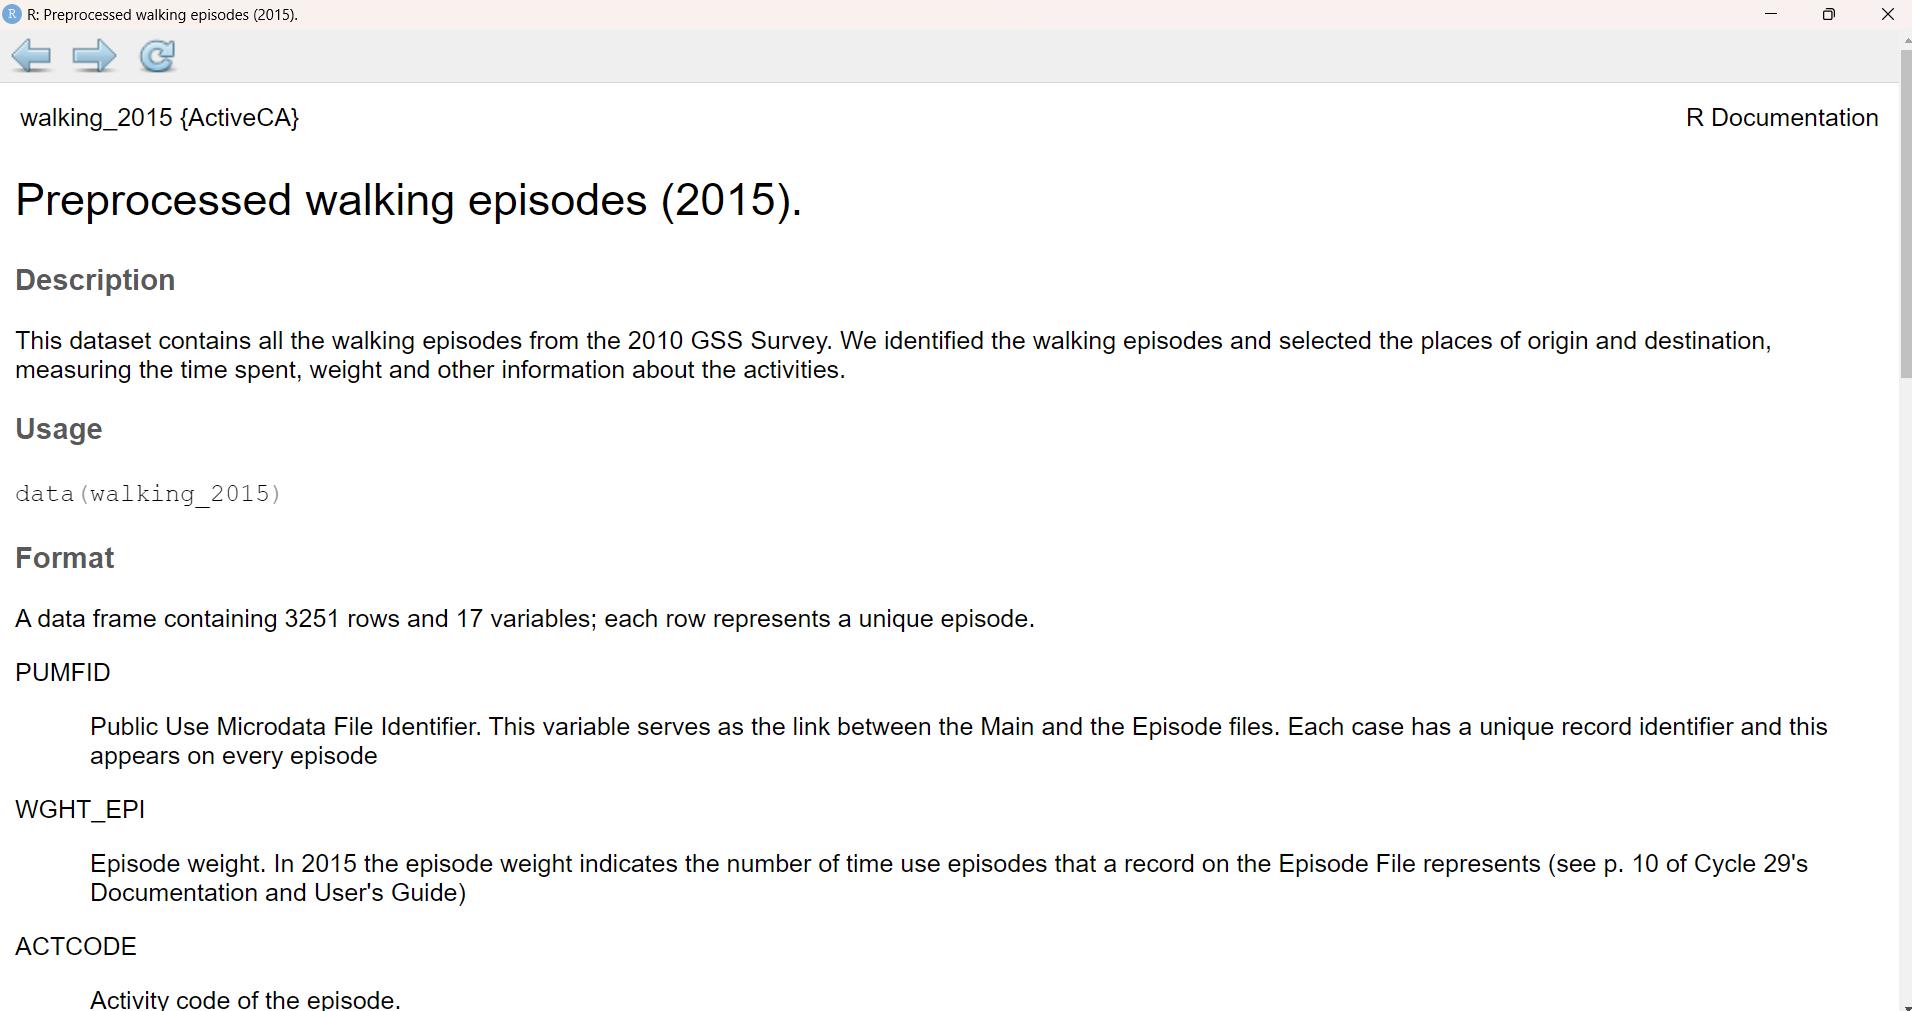
\includegraphics[width=1\linewidth]{Manuscript-figures/walking-2015-documentation} 

}

\caption{Documentation for the dataset of walking episodes from 2015.}\label{fig:walking_documentation}
\end{figure}

The code below shows how to load the walking episodes from the 2015 GSS
(Cycle 29):

\begin{Shaded}
\begin{Highlighting}[]
\FunctionTok{data}\NormalTok{(walking\_2015)}
\end{Highlighting}
\end{Shaded}

The GSS surveys apply a probability sampling methodology, in which each
episode or person selected in the sample represents several other
episodes or persons not in the sample. The number of episodes and
persons represented by a episode or person is determined by the weight
or weighting factor. Because of this, estimates of the number of
episodes or persons need to be calculated applying the corresponding
weighting factors.

For instance, to calculate the percentage of respondents from the 2015
GSS survey with active travel episodes, it is necessary to account for
the person's weight. In 2015, the weight variable is represented by
\texttt{WGHT\_PER.} The code below demonstrates how to obtain the
percentage of people with active travel episodes by age group. It uses
the \texttt{dplyr} package (Wickham et al. 2023) to manipulate the data.

The process begins by creating a dataset that sums the population by age
group. Then, it joins the 2015 episodes with the 2015 Main File. Note
that in both operations, the code sums the person weight variable
(\texttt{WGHT\_PER}) to obtain the correct population values. After
this, a new dataset, \texttt{Active\_percentage}, is created by merging
both previous datasets. The percentage of active travel episodes by age
group is calculated by dividing the total population by the population
with active trip episodes, then multiplying by 100 and rounding with 2
decimal places.

\begin{verbatim}
# Load the dplyr library for data manipulation
library('dplyr')

# Load the episodes dataset
data(gss_episodes) 

# Calculate the total population for each age group
Total_population <- gss_main_2015 |> 
  group_by(AGEGR10) |> 
  summarise(Total_population  = sum(WGHT_PER))

# Calculate the active population for each age group
Active_population <- gss_episodes |> 
      filter(YEAR == 2015) |> 
  left_join(gss_main_2015, by = c("PUMFID"="PUMFID")) |> 
  group_by(AGEGR10) |> 
  summarise(Active_population  = sum(WGHT_PER))

# Combine total and active population 
#and calculate the percentage
Active_percentage <- Total_population |> 
  left_join(Active_population, by = c("AGEGR10" = "AGEGR10")) |>
  mutate(
    Percentage = round(Active_population/Total_population*100,2))
\end{verbatim}

The result shows that the age group with the highest share of active
trips is those between 15 and 20 years old, with almost 37\%, followed
by those between 25 and 34 years old with around 33\%. There is a
significant drop in percentage for the following groups, with the
percentage falling to between 15\% and 18\% for the remaining age
groups.

\begin{longtable}[]{@{}lrrr@{}}
\toprule\noalign{}
AGEGR10 & Total\_population & Active\_population & Percentage \\
\midrule\noalign{}
\endhead
\bottomrule\noalign{}
\endlastfoot
15 to 24 years & 4511131 & 1641468.3 & 36.39 \\
25 to 34 years & 4956386 & 1644032.8 & 33.17 \\
35 to 44 years & 4734506 & 847769.9 & 17.91 \\
45 to 54 years & 5136125 & 790667.3 & 15.39 \\
55 to 64 years & 4831306 & 767064.0 & 15.88 \\
65 to 74 years & 3283969 & 559024.6 & 17.02 \\
75 years and over & 2312976 & 384358.6 & 16.62 \\
\end{longtable}

\subsection{Processed data set}\label{processed-data-set}

Table \ref{tab:processed-obs} displays the total number of records
processed for Main and Episode Files. For the Main Files, a total of
89,331 records were processed, referring to all records from the Time
Use Surveys from 1986 to 2015, that together represents more of
149,389,839 respondents (29,766,399 for 2015, 28,075,610 for 2010,
26,095,819 for 2005, 24,260,137 for 1998, 21,294,313 for 1992, and for
2005, 24,260,137 for 1998, and 21,294,313 for 1986). It also presents
the total cases of active trips episodes identified. In total 23,513
records with register of active travel activity. Together, these records
account for 44,316,110 episodes.

\begingroup\fontsize{10}{12}\selectfont

\begin{longtable}[t]{lrrr}
\caption{\label{tab:table_df_processed}\label{tab:processed-obs}Total number and weighted sum of records processed.}\\
\toprule
\multicolumn{2}{c}{ } & \multicolumn{2}{c}{Observations} \\
\cmidrule(l{3pt}r{3pt}){3-4}
Survey & Year & Count & Weighted\\
\midrule
 & 2015 & 17390 & 29766399\\
\nopagebreak
 & 2010 & 15390 & 28075610\\
\nopagebreak
 & 2005 & 19597 & 26095819\\
\nopagebreak
 & 1998 & 10749 & 24260137\\
\nopagebreak
 & 1992 & 9815 & 21294313\\
\nopagebreak
\multirow[t]{-6}{*}{\raggedright\arraybackslash Main} & 1986 & 16390 & 19897562\\
\cmidrule{1-4}\pagebreak[0]
 & 2022 & 1765 & 6041032\\
\nopagebreak
 & 2015 & 3496 & 6634387\\
\nopagebreak
 & 2010 & 4615 & 8516753\\
\nopagebreak
 & 2005 & 5866 & 7583838\\
\nopagebreak
 & 1998 & 1789 & 3606987\\
\nopagebreak
 & 1992 & 1635 & 3691918\\
\nopagebreak
\multirow[t]{-7}{*}{\raggedright\arraybackslash Episode} & 1986 & 4347 & 8241196\\
\bottomrule
\end{longtable}
\endgroup{}

Table \ref{tab:main-2015-processed} shows the first ten rows and first
six variables of the GSS PUMF 2015 Main File (Cycle 29), displayed in
\ref{tab:main-2015-unprocessed} before our processing. Table
\ref{tab:ep-2015-processed} presents the walking episodes for the record
identification number \texttt{10041} from the GSS PUMF 2015 Episode File
(Cycle 29), previously displayed in Table \ref{tab:ep-2015-unprocessed}.
Only the unique active travel episode appear in Table
\ref{tab:ep-2015-processed} since the records were filtered to select
cases with walking or cycling episodes. For both cases, Tables
\ref{tab:main-2015-processed} and \ref{tab:ep-2015-processed} contain
labeled variables, facilitating the interpretation of the data.

\begingroup\fontsize{8}{10}\selectfont

\begin{ThreePartTable}
\begin{TableNotes}
\item \textit{Note: } 
\item Legend: `PUMFID`: record identification. `WGHT\_PER`:  person weight. `SURVMNTH`: survey month of data collection. `AGEGR10`: age group of the respondent. `SEX`: sex of the respondent. `MARSTAT`: marital status of the respondent.
\end{TableNotes}
\begin{longtable}[t]{cccccc}
\caption{\label{tab:gss-processed-file-2015}\label{tab:main-2015-processed}Visualization of the first ten lines and first six columns of the Main File of the 2015 GSS.}\\
\toprule
PUMFID & WGHT\_PER & SURVMNTH & AGEGR10 & SEX & MARSTAT\\
\midrule
10000 & 616.6740 & July & 55 to 64 years & Male & Divorced\\
10001 & 8516.6140 & July & 55 to 64 years & Male & Married\\
10002 & 371.7520 & January & 45 to 54 years & Female & Married\\
10003 & 1019.3135 & March & 65 to 74 years & Female & Divorced\\
10004 & 1916.0708 & September & 25 to 34 years & Male & Single, never married\\
\addlinespace
10005 & 1952.2015 & April & 15 to 24 years & Male & Single, never married\\
10006 & 5761.5528 & August & 15 to 24 years & Male & Single, never married\\
10007 & 466.0426 & June & 55 to 64 years & Female & Widowed\\
10008 & 2479.2991 & February & 25 to 34 years & Female & Married\\
10009 & 1436.1641 & August & 65 to 74 years & Male & Widowed\\
\bottomrule
\insertTableNotes
\end{longtable}
\end{ThreePartTable}
\endgroup{}

\begingroup\fontsize{8}{10}\selectfont

\begin{ThreePartTable}
\begin{TableNotes}
\item \textit{Note: } 
\item Legend: `PUMFID`: record identification. `EPINO`: episode number. WGHT\_EPI: episode's weight. TUI\_01: activity code. DURATION: episode's duration. LOCATION: episode's location.
\end{TableNotes}
\begin{longtable}[t]{rrlrlll}
\caption{\label{tab:gss-processed-file-2015}\label{tab:ep-2015-processed}Visualization of the active travel episode for the record number `10041` of the 2015 GSS survey.}\\
\toprule
PUMFID & WGHT\_EPI & Activity & Duration & Origin & Destination & Mode\\
\midrule
10041 & 1353.818 & Transport to or from activity & 15 & Home & Home & Walking\\
\bottomrule
\insertTableNotes
\end{longtable}
\end{ThreePartTable}
\endgroup{}

\subsection{Descriptive statistics}\label{descriptive-statistics}

Considering GSS Cycles analyzed, we identified 23,513 episodes that
recorded active travel episodes, with trip duration ranging from 0 to
900 minutes, to twelve different destinations. \{ActiveCA\} includes all
these episodes ready for analysis. Table \ref{tab:table-01} presents
descriptive statistics on walking and cycling trips between 1986 and
2015, with measures of trip duration in minutes. The 1986 survey did not
include bicycle trips.

\begingroup\fontsize{10}{12}\selectfont

\begin{longtable}[t]{>{}llccccccc}
\caption{\label{tab:table-01}\label{tab:table-01}Descriptive statistics for episodes with active transport records}\\
\toprule
\multicolumn{2}{c}{ } & \multicolumn{7}{c}{Year} \\
\cmidrule(l{3pt}r{3pt}){3-9}
Mode & Statistic & 1986 & 1992 & 1998 & 2005 & 2010 & 2015 & 2022\\
\midrule
 & Maximum & 660 & 300 & 255 & 515 & 480 & 900 & 480\\
\nopagebreak
 & Mean & 21 & 21 & 12 & 12 & 13 & 18 & 19\\
\nopagebreak
 & Median & 15 & 10 & 5 & 10 & 10 & 10 & 15\\
\nopagebreak
 & Minimum & 1 & 1 & 1 & 0 & 0 & 5 & 5\\
\nopagebreak
\multirow[t]{-5}{*}{\raggedright\arraybackslash \textbf{Walking}} & Standard deviation & 31 & 25 & 17 & 16 & 17 & 27 & 24\\
\cmidrule{1-9}\pagebreak[0]
 & Maximum &  & 240 & 90 & 180 & 153 & 120 & 150\\
\nopagebreak
 & Mean &  & 28 & 24 & 20 & 19 & 25 & 40\\
\nopagebreak
 & Median &  & 15 & 15 & 15 & 10 & 20 & 30\\
\nopagebreak
 & Minimum &  & 5 & 2 & 1 & 1 & 5 & 5\\
\nopagebreak
\multirow[t]{-5}{*}{\raggedright\arraybackslash \textbf{Cycling}} & Standard deviation &  & 36 & 18 & 18 & 23 & 20 & 20\\
\bottomrule
\end{longtable}
\endgroup{}

Table \ref{tab:table-01} shows that, in general, the median values for
walking trips is 10 minutes, except for 1998 when the median was 5
minutes. In the case of cycling trips, the duration fluctuated over the
years, ranging from 10 to 20 minutes. The table also highlights very
high maximum values, particularly for walking trips, with recorded
episodes exceeding 4 hours in all cases.

Table \ref{tab:table-02} and \ref{tab:table-03} provide descriptive
statistics for the two modes of transportation, split by destination
categories, from 1986 to 1998 and from 2005 to 2015, respectively. In
Table \ref{tab:table-02}, one can observed that in 1986 and 1992,
walking trips destined for \texttt{home} had the highest medians.
However, by 1998, the highest medians shifted to trips to
\texttt{work\ or\ school}, a transition that also occurred for cycling
trips between 1992 and 1998. Table \ref{tab:table-03} indicates that the
median duration for walking trips to \texttt{home} and
\texttt{work\ or\ school} remained at 10 minutes.

\begingroup\fontsize{6}{8}\selectfont

\begin{ThreePartTable}
\begin{TableNotes}
\item \textit{Note: } 
\item 'Min' denotes the minimum time to reach the destination; 'Max' denotes the maximum time to reach the destination; '(\%)' indicates a percentage of the total time to reach the destination; 'Med' refers to the median time to reach the destination
\end{TableNotes}
\begin{longtable}[t]{ccccc>{}c|ccc>{}c|cccc}
\caption{\label{tab:table-02}\label{tab:table-02}Comparison of travel statistics by mode and destination: 1986, 1992, 1998}\\
\toprule
\multicolumn{2}{c}{ } & \multicolumn{4}{c}{1986} & \multicolumn{4}{c}{1992} & \multicolumn{4}{c}{1998} \\
\cmidrule(l{3pt}r{3pt}){3-6} \cmidrule(l{3pt}r{3pt}){7-10} \cmidrule(l{3pt}r{3pt}){11-14}
\multicolumn{1}{c}{\textbf{Destination}} & \multicolumn{1}{c}{\textbf{Mode}} & \multicolumn{1}{c}{\textbf{Min}} & \multicolumn{1}{c}{\textbf{Med}} & \multicolumn{1}{c}{\textbf{Max}} & \multicolumn{1}{c}{\textbf{(\%)}} & \multicolumn{1}{c}{\textbf{Min}} & \multicolumn{1}{c}{\textbf{Med}} & \multicolumn{1}{c}{\textbf{Max}} & \multicolumn{1}{c}{\textbf{(\%)}} & \multicolumn{1}{c}{\textbf{Min}} & \multicolumn{1}{c}{\textbf{Med}} & \multicolumn{1}{c}{\textbf{Max}} & \multicolumn{1}{c}{\textbf{(\%)}}\\
\midrule
 & Home &  &  &  &  & 5 & 20 & 240 & 55.7 & 2 & 15 & 90 & 51.6\\
\nopagebreak
 & Other's home &  &  &  &  & 5 & 10 & 145 & 19.7 & 2 & 10 & 80 & 15.7\\
\nopagebreak
\multirow[t]{-3}{*}{\centering\arraybackslash Cycling} & Work or school &  &  &  &  & 5 & 15 & 45 & 24.7 & 5 & 25 & 75 & 32.8\\
\cmidrule{1-14}\pagebreak[0]
 & Home & 1 & 15 & 330 & 46.3 & 1 & 15 & 300 & 60.5 & 1 & 5 & 255 & 51.9\\
\nopagebreak
 & Other's home & 1 & 10 & 660 & 42.6 & 1 & 5 & 135 & 18.7 & 1 & 5 & 120 & 27.8\\
\nopagebreak
\multirow[t]{-3}{*}{\centering\arraybackslash Walking} & Work or school & 1 & 10 & 450 & 11.1 & 2 & 10 & 60 & 20.9 & 1 & 10 & 75 & 20.3\\
\bottomrule
\insertTableNotes
\end{longtable}
\end{ThreePartTable}
\endgroup{}

\begingroup\fontsize{6}{8}\selectfont

\begin{ThreePartTable}
\begin{TableNotes}
\item \textit{Note: } 
\item 'Min' denotes the minimum time to reach the destination; 'Max' denotes the maximum time to reach the destination; '(\%)' indicates a percentage of the total time to reach the destination; 'Med' refers to the median time to reach the destination
\end{TableNotes}
\begin{longtable}[t]{ccccc>{}c|ccc>{}c|cccc}
\caption{\label{tab:table-03}\label{tab:table-03}Comparison of travel statistics by mode and destination: 2005, 2010, 2015}\\
\toprule
\multicolumn{2}{c}{ } & \multicolumn{4}{c}{2005} & \multicolumn{4}{c}{2010} & \multicolumn{4}{c}{2015} \\
\cmidrule(l{3pt}r{3pt}){3-6} \cmidrule(l{3pt}r{3pt}){7-10} \cmidrule(l{3pt}r{3pt}){11-14}
\multicolumn{1}{c}{\textbf{Destination}} & \multicolumn{1}{c}{\textbf{Mode}} & \multicolumn{1}{c}{\textbf{Min}} & \multicolumn{1}{c}{\textbf{Med}} & \multicolumn{1}{c}{\textbf{Max}} & \multicolumn{1}{c}{\textbf{(\%)}} & \multicolumn{1}{c}{\textbf{Min}} & \multicolumn{1}{c}{\textbf{Med}} & \multicolumn{1}{c}{\textbf{Max}} & \multicolumn{1}{c}{\textbf{(\%)}} & \multicolumn{1}{c}{\textbf{Min}} & \multicolumn{1}{c}{\textbf{Med}} & \multicolumn{1}{c}{\textbf{Max}} & \multicolumn{1}{c}{\textbf{(\%)}}\\
\midrule
 & Cultural venues & 10 & 10 & 15 & 0.3 & 10 & 25 & 30 & 1.0 & 15 & 15 & 15 & 0.5\\
\nopagebreak
 & Grocery store & 2 & 10 & 30 & 10.4 & 5 & 10 & 75 & 7.2 & 5 & 15 & 80 & 5.5\\
\nopagebreak
 & Health clinic &  &  &  &  &  &  &  &  & 10 & 15 & 90 & 1.9\\
\nopagebreak
 & Home & 1 & 15 & 180 & 48.4 & 1 & 10 & 135 & 48.8 & 5 & 20 & 120 & 46.4\\
\nopagebreak
 & Neighbourhood &  &  &  &  &  &  &  &  & 10 & 30 & 45 & 1.3\\
\nopagebreak
 & Other's home & 1 & 10 & 35 & 9.4 & 5 & 10 & 45 & 9.7 & 5 & 15 & 40 & 4.8\\
\nopagebreak
 & Outdoors & 5 & 15 & 45 & 6.0 & 3 & 10 & 115 & 2.6 & 15 & 30 & 30 & 1.0\\
\nopagebreak
 & Place of worship & 20 & 20 & 20 & 0.1 &  &  &  &  & 15 & 15 & 15 & 0.2\\
\nopagebreak
 & Restaurant & 5 & 15 & 35 & 2.8 & 10 & 15 & 153 & 1.7 & 10 & 20 & 60 & 3.0\\
\nopagebreak
 & Sport area &  &  &  &  &  &  &  &  & 10 & 15 & 15 & 2.0\\
\nopagebreak
\multirow[t]{-11}{*}{\centering\arraybackslash Cycling} & Work or school & 1 & 15 & 90 & 22.6 & 1 & 15 & 100 & 29.0 & 5 & 20 & 120 & 33.5\\
\cmidrule{1-14}\pagebreak[0]
 & Business &  &  &  &  &  &  &  &  & 5 & 10 & 30 & 0.2\\
\nopagebreak
 & Cultural venues & 5 & 10 & 40 & 0.6 & 2 & 10 & 40 & 0.7 & 5 & 15 & 40 & 1.5\\
\nopagebreak
 & Grocery store & 1 & 10 & 90 & 11.5 & 1 & 7 & 105 & 13.1 & 5 & 10 & 130 & 10.3\\
\nopagebreak
 & Health clinic &  &  &  &  &  &  &  &  & 5 & 10 & 130 & 0.9\\
\nopagebreak
 & Home & 0 & 10 & 515 & 43.0 & 0 & 10 & 270 & 41.4 & 5 & 10 & 900 & 44.0\\
\nopagebreak
 & Neighbourhood &  &  &  &  &  &  &  &  & 5 & 10 & 60 & 2.6\\
\nopagebreak
 & Other's home & 1 & 5 & 300 & 10.2 & 0 & 5 & 140 & 10.2 & 5 & 10 & 120 & 6.2\\
\nopagebreak
 & Outdoors & 1 & 5 & 295 & 3.4 & 0 & 10 & 480 & 5.0 & 5 & 10 & 135 & 3.1\\
\nopagebreak
 & Place of worship & 1 & 10 & 30 & 0.7 & 1 & 7 & 60 & 0.8 & 5 & 15 & 45 & 1.1\\
\nopagebreak
 & Restaurant & 0 & 5 & 85 & 9.9 & 1 & 7 & 153 & 11.0 & 5 & 10 & 120 & 9.0\\
\nopagebreak
 & Sport area &  &  &  &  &  &  &  &  & 5 & 10 & 45 & 3.3\\
\nopagebreak
\multirow[t]{-12}{*}{\centering\arraybackslash Walking} & Work or school & 0 & 10 & 175 & 20.7 & 0 & 10 & 150 & 17.9 & 5 & 10 & 190 & 17.8\\
\bottomrule
\insertTableNotes
\end{longtable}
\end{ThreePartTable}
\endgroup{}

\{ActiveCA\} also enables visual analysis of active travel in Canada
using traditional exploratory data analysis techniques. Figures
\ref{fig:figure-01} and \ref{fig:figure-02} show walking and cycling
trips from 1992 and 2015 through heat maps. These maps use color
gradients to represent the percentage of trips between various origins
and destinations, with darker colors indicating higher percentages and
lighter colors representing less frequent routes. For conciseness, we
omitted the heat maps for the other years analyzed.

In 1992, walking trips with \texttt{home} as both the origin and
destination made up the majority, accounting for about 30\% of all
walking trips. These trips often involved leisure activities, like short
walks or dog walking. Following this, trips from \texttt{home} to
\texttt{work\ or\ school} comprised 18\% of walking trips. Overall,
\texttt{home} emerged as a crucial hub, either as an origin or
destination, with only 5\% of trips not involving \texttt{home.} By
2015, \texttt{home} remained a significant node, but new locations
distributed the proportion of trips to areas not considered in 1992. In
2015, the highest proportion of trips were from \texttt{home} to
\texttt{work\ or\ school} (12\%) and vice versa (11\%). \texttt{home} to
\texttt{home} accounted for 8\% of trips, and \texttt{grocery\ stores}
became a notable destination for those leaving \texttt{home} (6\%),
surpassing trips to \texttt{other\textquotesingle{}s\ home} (4\%).

\begin{figure}

{\centering 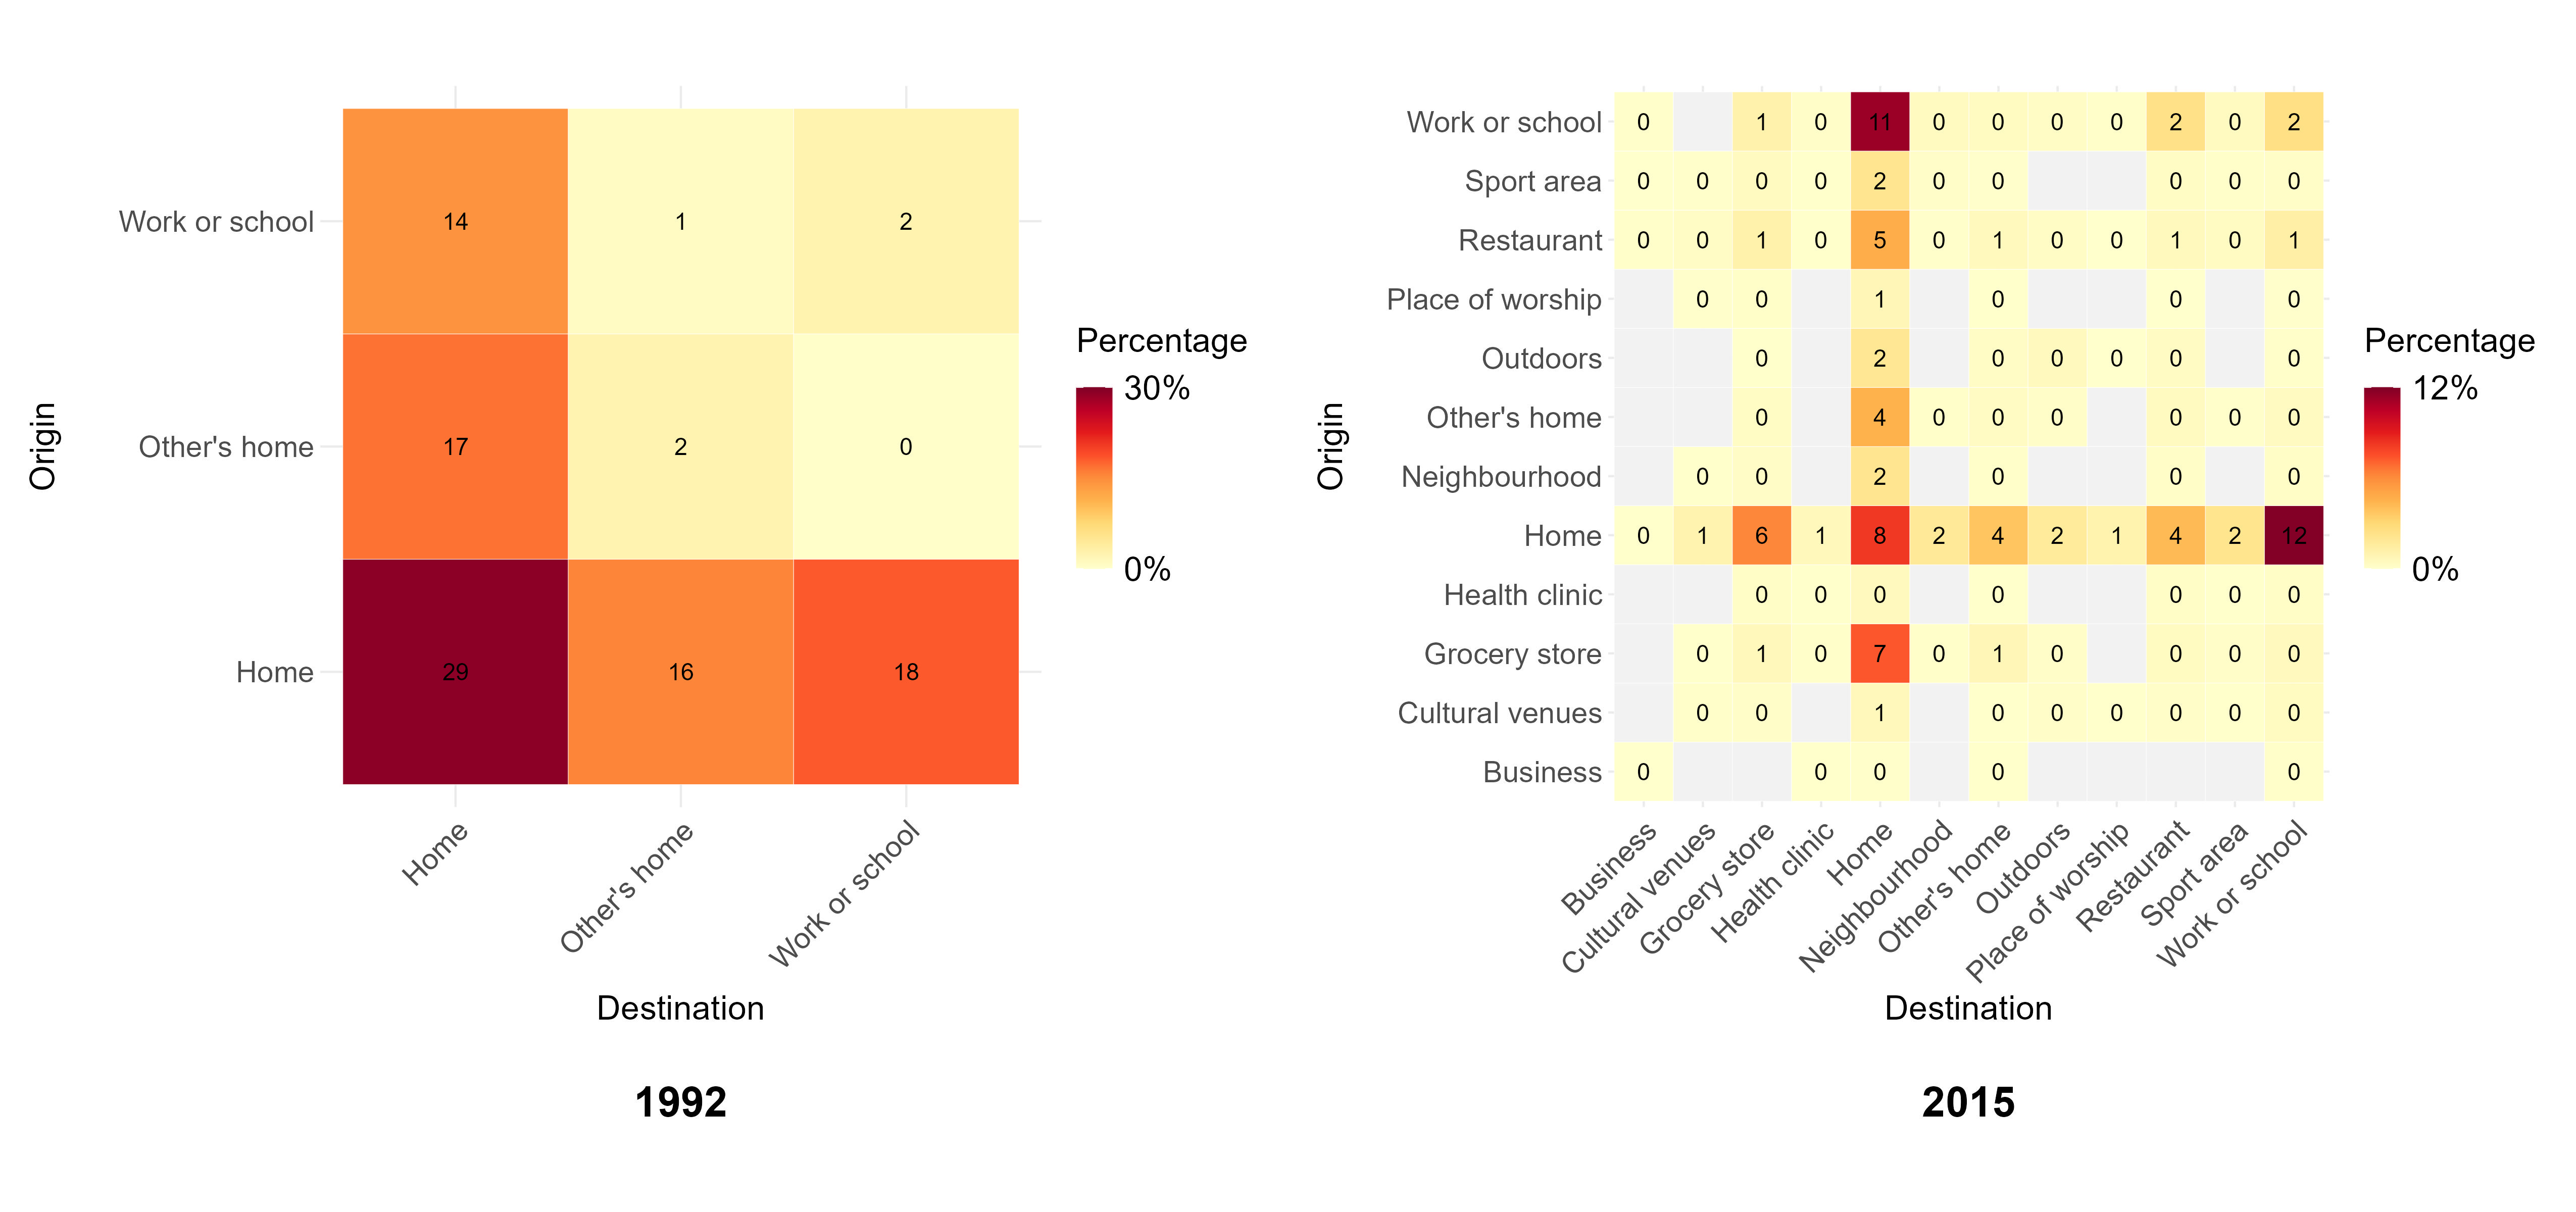
\includegraphics[width=1\linewidth]{Manuscript-figures/walking_hm_fig} 

}

\caption{Percentage of walking trips categorized by origin and destination}\label{fig:figure-01}
\end{figure}

For cycling trips, Figure \ref{fig:figure-02}, shows that in 1992, when
this mode of transportation was first included as an activity, the
majority of trips were from \texttt{home} to \texttt{work\ or\ school},
accounting for about 25\% of cases. This pattern remained in 2015, with
these trips representing 30\% of the cases. However, a notable change
occurred in \texttt{home} to \texttt{home} trips, which decreased
significantly from 19\% in 1992 to 5\% in 2015.

\begin{figure}

{\centering 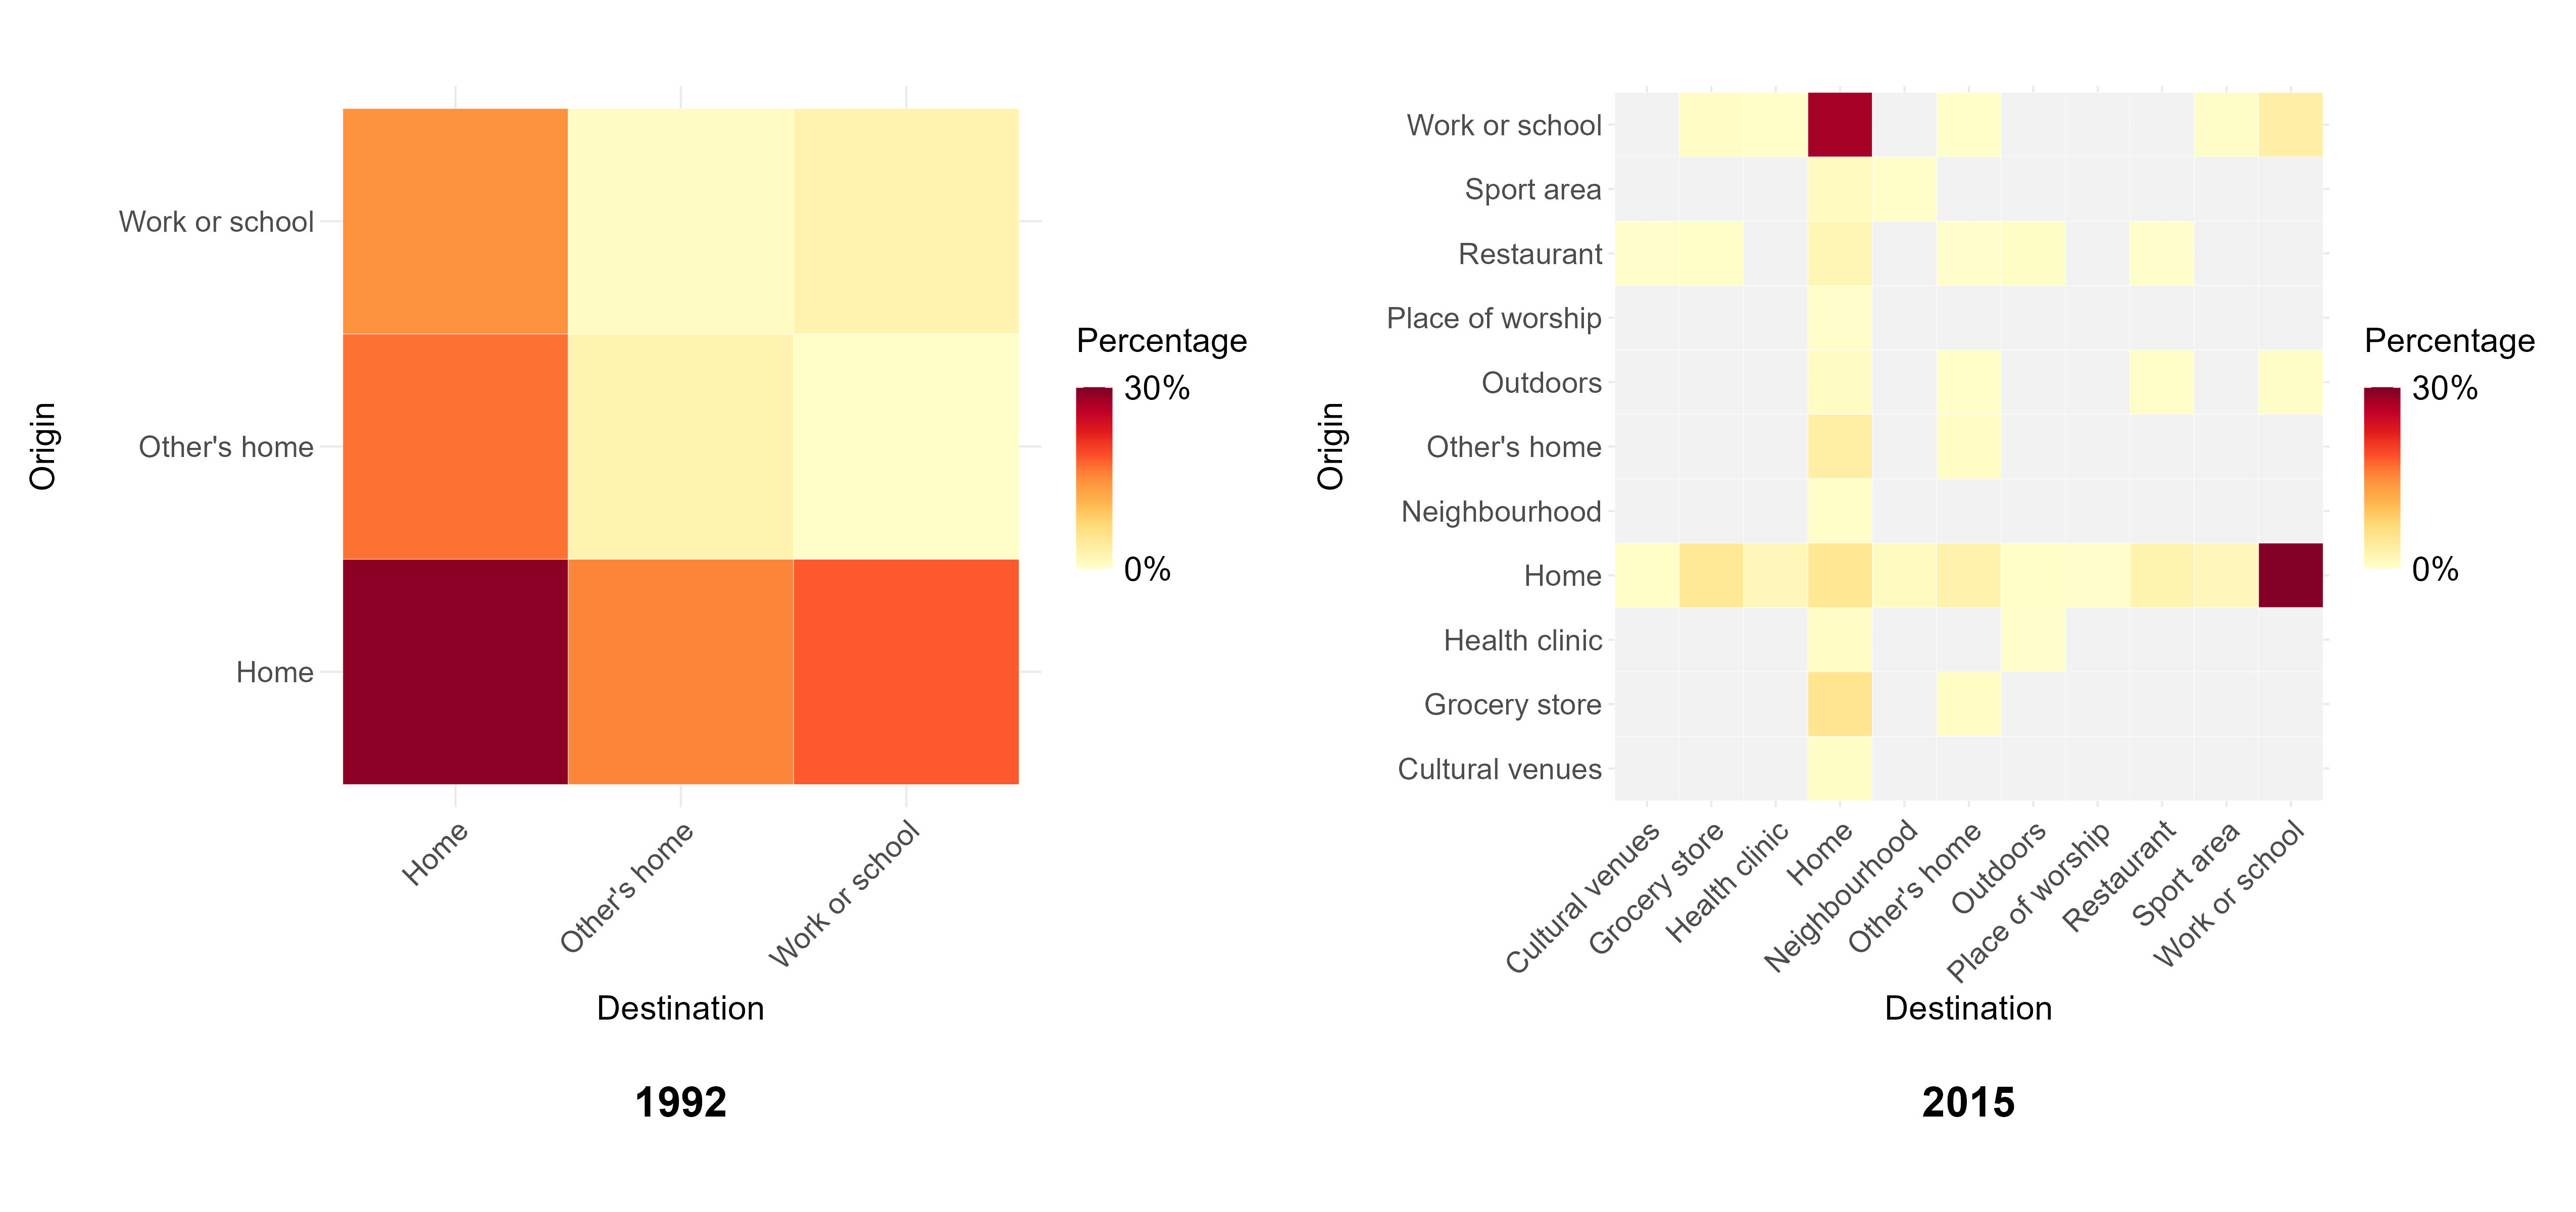
\includegraphics[width=1\linewidth]{Manuscript-figures/cycling_hm_fig} 

}

\caption{Percentage of cycling trips categorized by origin and destination}\label{fig:figure-02}
\end{figure}

\{ActiveCA\} also enables obtaining insights from the main processed
files. Figure \ref{fig:figure-stress} present how the level of stress
varied among respondents depending on their marital status in 2015.
According to this plot, married respondents reported the highest level
of stress, relating to feel stressed every day, with 17\% of possible
cases.

\begin{figure}

{\centering 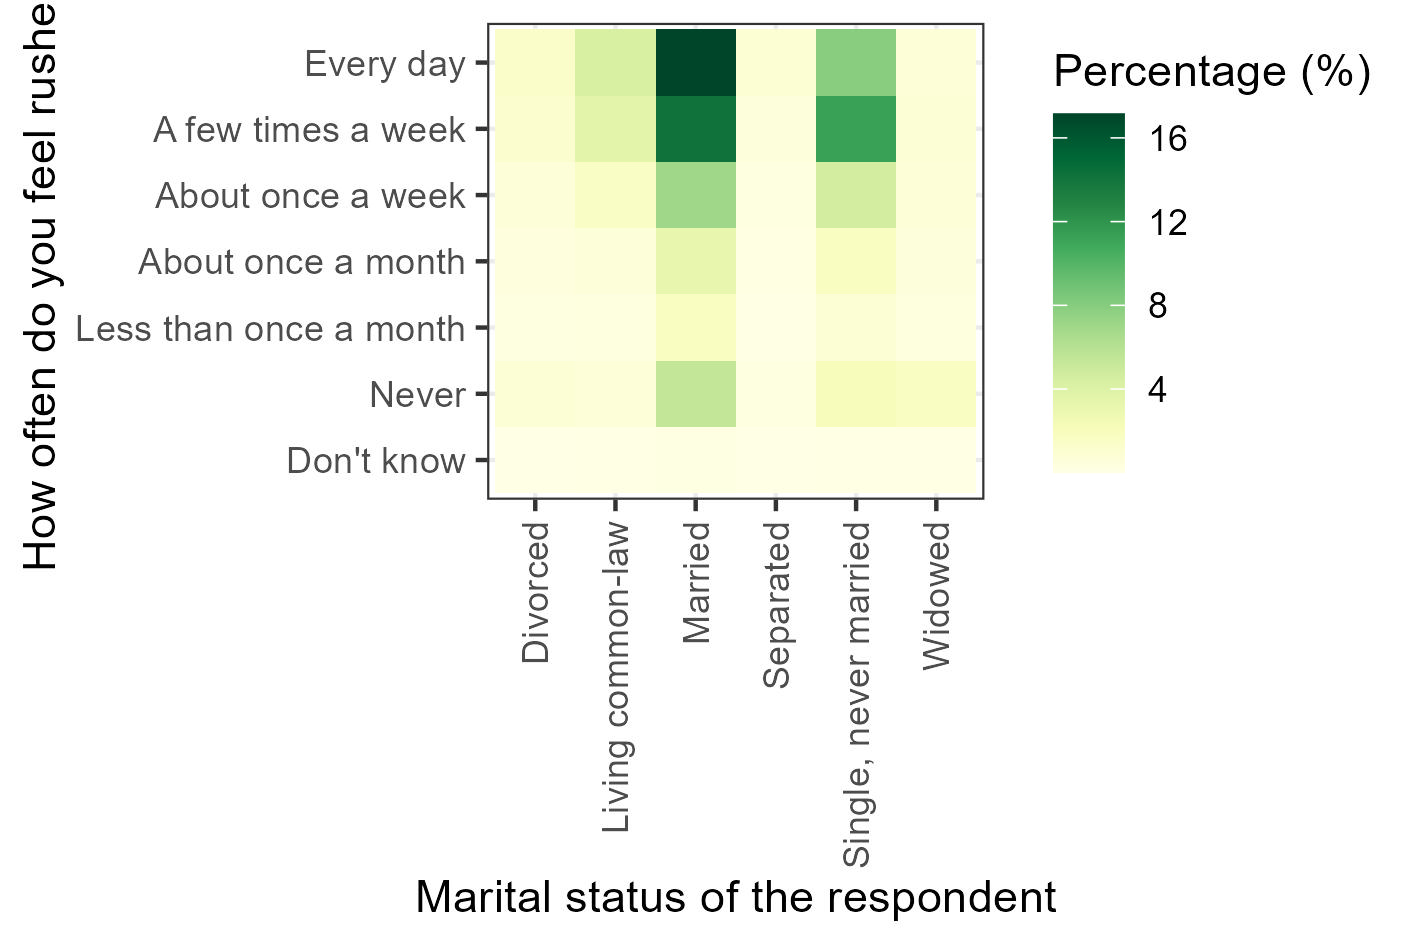
\includegraphics[width=1\linewidth]{Manuscript-figures/main_stress_figure} 

}

\caption{Level of stress among respondents of different marital statuses (2015).}\label{fig:figure-stress}
\end{figure}

\section{Python integration}\label{python-integration}

\{ActiveCA\} also provides a Jupyter Notebook containing a Python script
that demonstrates how to read R data files (.rda) and convert them into
Pandas DataFrames. This process allows users to work with and utilize
the datasets available in \{ActiveCA\} within a Python project.

\section{Concluding remarks}\label{concluding-remarks}

This paper presents \{ActiveCA\}, an open data product that provides
analysis-ready data from Cycles 2 (1986), 7 (1992), 12 (1998), 19
(2005), 24 (2010), and 29 (2015) of the GSS surveys on active travel in
Canada. In the form of an \texttt{R} data package, \{ActiveCA\} was
developed after collecting, cleaning, and processing the survey data,
providing information on origins, destinations, and duration of active
travel, as well other information.

It is important to remark that the present version of \{ActiveCA\}
covers all Canadian time use surveys up to 2015. While the most recent
time use survey was carried out in 2022 (Wray 2024), the Public Use
Microdata Files are currently unavailable, and at the moment it is
estimated that they will only be published in the later part of 2025.
The \texttt{R} package will be updated once these files become
available.

The value of \{ActiveCA\} lies in its transparency, accessibility, and
ease of use, which facilitates the addition of complementary data sets
in the future. \texttt{R} users can seamlessly explore GSS walking and
cycling episodes, with the option to suggest enhancements to the package
as needed. This article adopts the structure proposed by Anastasia and
Páez (2023), whose work provided essential guidance for the creation of
this package. Similarly, we aim to contribute to the academic community
by promoting transparent research practices that encourage replication
and innovation in related fields. We believe that \{ActiveCA\} will
serve as a basis for further research on GSS and for the integration of
additional data by the authors or the wider open source community.

\section{Declaration of Conflicting
Interests}\label{declaration-of-conflicting-interests}

The author(s) declared no potential conflicts of interest with respect
to the research, authorship, and/or publication of this article.

\section{Funding}\label{funding}

The author(s) disclosed receipt of the following financial support for
the research, authorship, and/or publication of this article: This work
was supported by the Social Sciences and Humanities Research Council of
Canada (\emph{More description about the funding source after the review
process}).

\section{ORCID}\label{orcid}

Author 1

Author 2

Author 3

\section{Data availability statement}\label{data-availability-statement}

The \{ActiveCA\} R data package can be found and installed on Github
(\emph{link}).

For review purposes, the package is currently available as a tar.gz file
that can be installed by R. The file can be obtained from this anonymous
location:

\url{https://user.fm/files/v2-3d261d0b2aa47fcad096cd9e49fd5cf8/ActiveCA.zip}

\section*{References}\label{references}
\addcontentsline{toc}{section}{References}

\phantomsection\label{refs}
\begin{CSLReferences}{1}{0}
\bibitem[\citeproctext]{ref-arribas-bel2021}
Arribas-Bel, Dani, Mark Green, Francisco Rowe, and Alex Singleton. 2021.
{``Open Data Products-A Framework for Creating Valuable Analysis Ready
Data.''} \emph{Journal of Geographical Systems} 23 (4): 497--514.
\url{https://doi.org/10.1007/s10109-021-00363-5}.

\bibitem[\citeproctext]{ref-brunsdon_opening_2021}
Brunsdon, Chris, and Alexis Comber. 2021. {``Opening Practice:
Supporting Reproducibility and Critical Spatial Data Science.''}
\emph{Journal of Geographical Systems} 23 (4): 477--96.
\url{https://doi.org/10.1007/s10109-020-00334-2}.

\bibitem[\citeproctext]{ref-statisticscanada2022}
Canada, Statistics. 2022. {``Time Use Survey.''}
\url{https://www23.statcan.gc.ca/imdb/p2SV.pl?Function=getSurvey&amp;SDDS=4503}.

\bibitem[\citeproctext]{ref-statisticscanada2024}
---------. 2024. {``Statistics Canada: Canada's National Statistical
Agency.''} \url{https://www.statcan.gc.ca/en/start}.

\bibitem[\citeproctext]{ref-kimFacing2024}
Kim, Sang-O, Matthew Palm, Soojung Han, and Nicholas J. Klein. 2024.
{``Facing a Time Crunch: {Time} Poverty and Travel Behaviour in
{Canada}.''} \emph{Transportation Research Part D: Transport and
Environment} 126 (January): 104028.
\url{https://doi.org/10.1016/j.trd.2023.104028}.

\bibitem[\citeproctext]{ref-lachapelleLonger2016}
Lachapelle, Ugo, and Diogo Gianini Pinto. 2016. {``Longer or More
Frequent Walks: {Examining} the Relationship Between Transit Use and
Active Transportation in {Canada}.''} \emph{Journal of Transport \&
Health}, Special {Issue}: {Public} {Transport} and {Health}, 3 (2):
173--80. \url{https://doi.org/10.1016/j.jth.2016.02.005}.

\bibitem[\citeproctext]{ref-mccurdySupport2023}
McCurdy, Ashley, Guy Faulkner, Christine Cameron, Christa
Costas-Bradstreet, and John C. Spence. 2023. {``Support for {Active}
{Transport} {Policy} {Initiatives} {Among} {Canadian} {Adults}: {The}
{Canadian} {National} {Active} {Transportation} {Survey}.''}
\emph{Active Travel Studies} 3 (2).
\url{https://doi.org/10.16997/ats.1450}.

\bibitem[\citeproctext]{ref-paez_open_2021}
Páez, Antonio. 2021. {``Open Spatial Sciences: An Introduction.''}
\emph{Journal of Geographical Systems} 23 (4): 467--76.
\url{https://doi.org/10.1007/s10109-021-00364-4}.

\bibitem[\citeproctext]{ref-soukhov2023}
Soukhov, Anastasia, and Antonio Páez. 2023. {``TTS2016R: A Data Set to
Study Population and Employment Patterns from the 2016 Transportation
Tomorrow Survey in the Greater Golden Horseshoe Area, Ontario,
Canada.''} \emph{Environment and Planning B: Urban Analytics and City
Science} 50 (2): 556--63.
\url{https://doi.org/10.1177/23998083221146781}.

\bibitem[\citeproctext]{ref-spinneyTransport2009}
Spinney, J. E. L., D. M. Scott, and K. B. Newbold. 2009. {``Transport
Mobility Benefits and Quality of Life: {A} Time-Use Perspective of
Elderly {Canadians}.''} \emph{Transport Policy} 16 (1): 1--11.
\url{https://doi.org/10.1016/j.tranpol.2009.01.002}.

\bibitem[\citeproctext]{ref-dplyr2023}
Wickham, Hadley, Romain François, Lionel Henry, Kirill Müller, and Davis
Vaughan. 2023. \emph{Dplyr: A Grammar of Data Manipulation}.
\url{https://dplyr.tidyverse.org}.

\bibitem[\citeproctext]{ref-wray2024}
Wray, Dana. 2024. {``Telework, Time Use, and Well-Being: Evidence from
the 2022 Time Use Survey.''}
\url{https://www150.statcan.gc.ca/n1/daily-quotidien/240605/dq240605a-eng.htm}.

\end{CSLReferences}

\end{document}
